\documentclass[specialist, substylefile = spbureport.rtx,
    subf,href,colorlinks=true, 12pt]{disser}

% \usepackage[a4paper, mag=1000, includefoot,
%     left=2cm, right=1.5cm, top=2cm, bottom=2cm, headsep=1cm, footskip=1cm]{geometry}

\usepackage[a4paper, top=2cm, bottom=2cm, left=2cm, right=2cm]{geometry}

\usepackage[T1,T2A]{fontenc}

\usepackage{graphicx}
\graphicspath{ {images/} }
\usepackage{amsmath}
\usepackage{amsfonts}
\usepackage{amsthm} %for \newtheorem*
\usepackage[english,russian]{babel}

% \pagestyle{plain}

\newtheorem*{definition}{Определение}
\newtheorem*{example}{Пример}
\newtheorem*{hypothesis}{Гипотеза}
\newtheorem*{question}{Вопрос}
\newtheorem*{algorithm}{Алгоритм}

\newcommand{\rank}{\mathsf{rank}\ }
\newcommand{\T}{\mathcal{T}}
\newcommand{\F}{\mathsf{F}}
\newcommand{\MF}{\vec{\F}}
\newcommand{\sfS}{\mathsf{S}}
\newcommand{\sfR}{\mathsf{R}}
\newcommand{\MS}{\vec{\sfS}}
\newcommand{\MSE}{\mathsf{MSE}}
\newcommand{\SSA}{\mathsf{SSA}}
\newcommand{\MSSA}{\mathsf{MSSA}}
\newcommand{\ProjSSA}{\mathsf{ProjSSA}}
\newcommand{\mean}{\mathsf{mean}}
\newcommand{\X}{\mathbf{X}}
\newcommand{\wX}{\overset{\wedge}{\X}}






\institution{Санкт-Петербургский государственный университет\\
    Математико-механический факультет\\
    Кафедра Статистического Моделирования
}
\title{«Научно-исследовательская работа» (семестр 6)}
\topic{Поддерживающие временные ряды в MSSA}
\author{Ткаченко Егор Андреевич}
\group{группа 19.Б04-мм}
\sa       {Голяндина Нина Эдуардовна}
\sastatus {к.\,ф.-м.\,н., доцент}
\city{Санкт-Петербург}
\date{2022}


\begin{document}

    \maketitle
    \pagebreak
    \tableofcontents
    \pagebreak

    \intro
        Полезность умения строить прогнозы не нуждается в доказательстве. Прогноз временных рядов может использоваться в прогнозе погоды, приливов, спроса на товары и многом другом.
         
        С помощью книги \cite{SSA_with_R} был изучен базовый $\SSA$, разложение рядов, заполнение пробелов в данных, прогноз и базовый $\MSSA$. Для работы с временными рядами и их прогнозом использовался пакет Rssa. Проведены эксперименты с простейшими моделями сигналов для изучения связи между согласованностью сигналов и поддерживающими рядами.



        % После этого я изучал 
    % \chapter{обозначения}
    \section{Определения}
        Вещественным временным рядом длины $N$ называется вектор
        $$\F = (f_0, \dots, f_{N - 1}),\ f_j \in \mathbb{R}.$$

        Многомерным временным рядом $\MF$ называется набор $s$ временных рядов $\F^{(p)}$ длин $N_p$:
        $$\MF = \{\F^{(p)} = (f^{(p)}_0, \dots, f^{(p)}_{N_p - 1}),\ p=1, \dots, s\}.$$

        $L$-траекторная матрица (или просто траекторная матрица) ряда $\F$ имеет структуру ганкелевой матрицы, а ее столбцами являются отрезки длины L ряда $\F$
        $$\T_{\SSA}(\F) =
        \begin{pmatrix}
            f_0     & f_1    & \dots  & f_{K-1} \\
            f_1     & f_2    & \dots  & f_K     \\
            \vdots  & \vdots & \ddots & \vdots  \\
            f_{L-1} & f_L    & \dots  & f_{N-1} \\
        \end{pmatrix}.$$
        $L$-траекторная матрица многомерного ряда $\MF$ состоит из горизонтально склеенных траекторных матриц рядов $\F^{(p)} \in \MF$:
        $$\T_{\MSSA}(\MF) = [\T_{\SSA}(\F^{(1)}): \dotso :\T_{\SSA}(\F^{(s)})].$$
        Из траекторной матрицы можно восстановить ряд. Из любой матрицы подходящего размера можно получить траекторную матрицу проектированием на пространство ганкелевых матриц (или склеенных горизонтально ганкелевых матриц для многомерного случая).

        Ранг ряда равен рангу его траекторной матрицы:
        $$\rank \F = \rank \T_{\SSA}(\F),\qquad \rank \MF = \rank \T_{\MSSA}(\MF).$$

        


    \section{Применение SSA и MSSA}

        Алгоритмы $\SSA$ и $\MSSA$ могут быть применены для аппроксимации временного ряда рядом конечного ранга.

        \begin{algorithm}\ \\
            \textbf{Вход:} Ряд $\F$ для $\SSA$ или многомерный ряд $\MF$ для $\MSSA$,
            длина окна $L \leq N$ для $\SSA$ или $L \leq N_p, \forall N_p$ для $\MSSA$,
            ранг аппроксимирующего ряда r.

            \begin{enumerate}
                \item[1] Вложение. Временной ряд переводится в L-траекторную матрицу $\X$
                    $$\X = \T_{\SSA}(\F) \text{ для $\SSA$,\qquad } \X = \T_{\MSSA}(\MF) \text{ для $\MSSA$.}$$
                \item[2] Сингулярное разложение. Методом SVD матрица $\X$ раскладывается на сумму $d$ матриц 
                $\X_i = \sqrt{\lambda_i}U_iV_i^T$, где $d = \rank \X = \rank \X\X^T \leq L$,
                $\lambda_i$ --- собственные числа матрицы $\X\X^T$ ($\lambda_1 \geq \dotso \geq \lambda_L \geq 0$),
                $U_i$ --- собственные вектора матрицы $\X\X^T$,
                $V_i = \X^T U_i / \sqrt{\lambda_i}$ --- факторные вектора матрицы $\X$.
                \item[3] Группировка. Множество индексов $\{1, \dots, d\}$ делится на $m$ непересекающихся множеств $I_1 ,\dots, I_m$. Далее для каждого множества индексов (пусть $I = {i_1, \dots, i_t}$) получается матрица $\X_I = \X_{i_1} + \dots + \X_{i_t}$.\\
                Для аппроксимации рядом конечного ранга $r$, понадобится множество из первых $r$ индексов $\{1, \dots, r\}$, соответствующую ему матрицу обозначу $\wX_r = \X_1 + \dots + \X_r$.
                \item[4] 
                Сгруппированные матрицы $\X_{I_j}$ восстанавливаются в ряды ($\SSA$) или многомерные ряды ($\MSSA$).
                Для получения аппроксимирующего ряда нужно восстановить его из матрицы $\wX_r$.
            \end{enumerate}
            \textbf{Выход:} Аппроксимирующий ряд $\overset{\wedge}{\F}_r$ конечного ранга r.
        \end{algorithm}

    \section{ЛРФ}
        Линейная рекуррентная формула (ЛРФ) выражает каждый член последовательности через линейную комбинацию предыдущих членов.

        Ряд $\F$ длины $N$ --- управляемый ЛРФ, если существуют такие $a_1, \dotso, a_d$, что:
        $$f_{i+d} = \sum_{k=1}^d a_k f_{i+d-k},\ 0 \leq i \leq N - 1 - d,\ a_d \neq 0,\ t < N - 1.$$
        Важно отметить, что ряд конечного ранга является управляемым ЛРФ \cite[2.1.2.2, стр. 35]{SSA_with_R}.
        
        

        Вещественный временной ряд $\F$, управляемый ЛРФ, естественным образом прогнозируется на одну точку:
        $$\overset{\sim}{f}_{N} = \sum_{k=1}^{L-1} a_k f_{N-k}.$$
        Но тогда его можно прогнозировать и на любое количество точек.
        % $$\overset{\sim}{\F}_{N_p} = (\overset{\sim}{f}_{N_p}, \dots, \overset{\sim}{f}_{N_p + \overset{\sim}{N}_p - 1}), \overset{\sim}{f_j} \in \mathbb{R}.$$
        % Также ряд управляемый ЛРФ, естественным образом можно прогнозировать на одно значение, а значит и на любое количество значений.

        % \begin{block}{Коэффициенты ЛРФ $a_1, \dotso, a_{L-1}$}
        %     $$(a_1, \dotso, a_{L-1}) = \mathcal{R}_L=\frac{1}{1-\sum_{j=1}^r \pi(U_j)^2} \sum_{j=1}^r \pi(U_j) \underline{U_j},$$
        %     где $\pi(U_j)$ --- последняя координата вектора $U_j$,\\ $\underline{U_j}$ --- вектор $U_j$ без последней координаты.
        % \end{block}



    \chapter{Постановка задачи}

        Пусть имеется временной ряд $\F^{(1)} = \sfS^{(1)} + \sfR^{(1)}$, где сигнал $\sfS^{(1)}$ --- ряд управляемый ЛРФ, шум~$\sfR^{(1)}$ --- ряд без структуры. Рассмотрим задачу прогнозирования $\sfS^{(1)}$. Эта задача уже решается методом $\SSA$, но как можно улучшить прогноз?

        Пусть помимо ряда $\F^{(1)}$ имеется временной ряд $\F^{(2)} = \sfS^{(2)} + \sfR^{(2)}$.
        Если структура сигналов $\sfS^{(1)}$ и $\sfS^{(2)}$ похожа, то использование ряда $\F^{(2)}$ может улучшить прогноз сигнала $\sfS^{(1)}$, потому что второй ряд дает алгоритму больше данных, которые могут улучшить ЛРФ.
        Возможность такого улучшения прогноза подтверждена \cite[4.3.3.3, стр. 216]{SSA_with_R}.
        Но второй ряд может сделать прогноз хуже, если структура его сигнала отличается от первого.

        Простейший пример похожих по структуре сигналов --- гармонические колебания с одинаковыми периодом. Они даже могут быть смещены по фазе или иметь разную амплитуду.

        Для объективной оценки качества прогноза будем использовать среднюю квадратичную ошибку.
        $$\mathsf{MSE(\overset{\sim}{S},\ S)} = \frac{1}{N_{f}} \sum_{i = N}^{N + N_{f} - 1} (\overset{\sim}{s}_i - s_i)^2,$$
        где $\overset{\sim}{\sfS}$ --- прогноз сигнала $\sfS$ на $N_{f}$ точек, $N$ --- длина прогнозируемого сигнала $\sfS$.
    

        Ряд $F^{(2)}$ называется поддерживающим для прогноза, если прогноз с его использованием лучше чем без него, т.е.
    
        $$\MSE(\overset{\sim}{\sfS}_{\MSSA},\ \sfS^{(1)}) < \MSE(\overset{\sim}{\sfS}_{\SSA},\ \sfS^{(1)}).$$
        Такое определение можно применить только в экспериментах с известным продолжением ряда. На практике не с чем сравнить прогноз, поэтому появляется вопрос. Как понять, что ряд поддерживающий не зная продолжения прогнозируемого ряда? Помочь ответить на этот вопрос может понятие согласованности.

        Сигналы $\sfS^{(1)}$, $\sfS^{(2)}$ называются полностью согласованными, если ранг $r_{1,2} = r_1 = r_2$ и полностью несогласованными, если $r_{1,2} = r_1 + r_2$, где $r_1 = \rank \sfS^{(1)}$, $r_2 = \rank \sfS^{(2)}$, $r_{1,2} = \rank \MS = \rank \{\sfS^{(1)}, \sfS^{(2)}\}.$

    % \section{Примеры}
    %     когда следует ожидать, что $\MSSA$ лучше
        % \begin{example}

        %     \begin{tabular}{lll}
        %     & $s^{(i)}_j = A_i\cos(\frac{2\pi j}{T_i})$ & $s^{(i)}_j = A_i\exp(j\lambda_i)$ \\
        %     Согласованные:  & $T_1 = T_2 \neq 2$ & $\lambda_1 = \lambda_2$
        %     \\
        %     Несогласованные:& $2 \neq T_1 \neq T_2 \neq 2$ & $\lambda_1 \neq \lambda_2$
        %     \end{tabular}
        % \end{example}

    \chapter{Численные эксперименты}
        
    \section{Первый эксперимент: выбор компонент для MSSA}
        Гипотеза: когда сигналы похожи, их можно считать согласованными и лучше использовать (при прогнозе или восстановлении сигнала) ранг равный рангу одного сигнала. Когда сигналы отличаются, их следует считать не согласованными и использовать ранг равный сумме рангов сигналов.

        Выберем в качестве первого ряда простой сигнал, зависящий от параметра (например, у косинуса параметр --- период) с аддитивным гауссовым шумом с дисперсией $\sigma_1^2 = 0.2^2$.
        Второй ряд будет простым сигналом того же вида, с несколько отличающимся параметром и без шума.
        Восстановим и спрогнозируем первый ряд с помощью $\SSA$, $\MSSA$ считая ряды согласованными и $\MSSA$ считая ряды несогласованными.

        Для устойчивости результатов, повторим это 50 раз и усредним ошибки.

        Назовем относительной ошибкой прогноза (восстановления) значение $$\displaystyle \frac{error_{\SSA} - error_{\MSSA}}{error_{\SSA} + error_{\MSSA}},$$ где $error_{\SSA}, error_{\MSSA}$ --- ошибки прогноза (восстановления) методами $\SSA$ и $\MSSA$ соответственно.
        
        Значения относительной ошибки легко расположить на графике (она принимает значения от -1 до 1). По значению относительной ошибки легче понять, какой метод лучше (не надо сравнивать два значения ошибок, которые просто положительны и могут быть любых порядков). Но относительную ошибку нельзя считать когда $error_{\SSA} = error_{\MSSA} = 0$.
        
        Как интерпретировать значения относительной ошибки? 
        \begin{itemize}
            \item значения больше $0$ значат, что что $\MSSA$ лучше $\SSA$;
            \item значения меньше $0$ значат, что что $\MSSA$ хуже $\SSA$;
            \item значения около $0$ значат что ошибки примерно равны;
            \item значения далеко от $0$ значат, что ошибки сильно отличаются.
        \end{itemize}

        Все сигналы в этом и следующих экспериментах будут нормироваться, чтобы амплитуда сигнала не влияла на ошибки прогноза и восстановления. Например, для косинуса: $s_j^{(i)} = A \cos(\frac{2\pi j}{T_i})$, где $A$ --- такая константа, что $\mean(|s_j^{(i)}|) = 1$.


    \subsection{Сигнал косинус}
        Сигнал $\sfS^{(1)}$ --- косинус с периодом $T_1 = 8$.
        Сигналы $\sfS^{(2)}$ --- косинусы с периодами $T_2 \in \{8$, $8.02$, $8.04$, $8.06$, $8.08$, $8.1$, $8.15\}$.

        Ранг косинуса равен 2, поэтому для $\MSSA$ используются первые 2 или первые 4 компоненты разложения, а для $\SSA$ только 2.

        \begin{figure}[h]
            \centering
            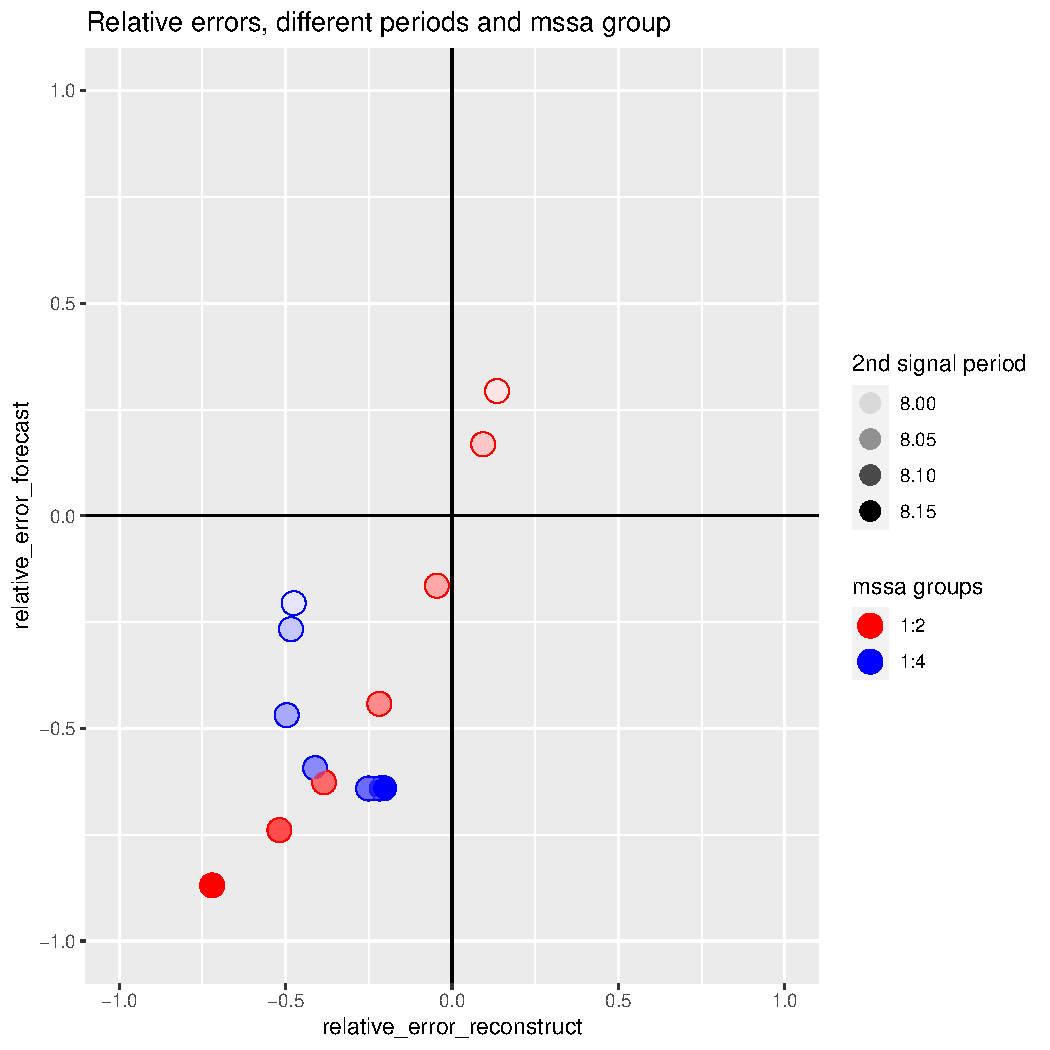
\includegraphics[width=\textwidth]{experiment_1_cos.pdf}
            \caption{Зависимость относительных ошибок от разницы сигналов и выбора ранга для $\MSSA$.}
            \label{fig:exp1_cos}
        \end{figure}

        На рис. \ref{fig:exp1_cos} видим подтверждение гипотезы для косинусов: с увеличением разницы рядов использование четырех компонент становится лучше и для прогноза и для восстановления сигнала.

    \subsection{Сигнал экспонента (показательная функция)}
        Функция для сигналов --- $s^{(i)}_j = A \exp(j\lambda_i)$.
        Сигнал $\sfS^{(1)}$ --- нормированная показательная функция c $\lambda_1 = 0.005$.
        Сигналы $\sfS^{(2)}$ --- нормированная показательная функция c $\lambda_2 \in \{0.005$, $0.0075$, $0.01$, $0.0125$, $0.015$, $0.02$, $0.025$, $0.03\}$.

        Ранг показательной функции равен 1, поэтому для $\MSSA$ используется первая или первые 2 компоненты разложения, а для $\SSA$ только первая.

        \begin{figure}[h]
            \centering
            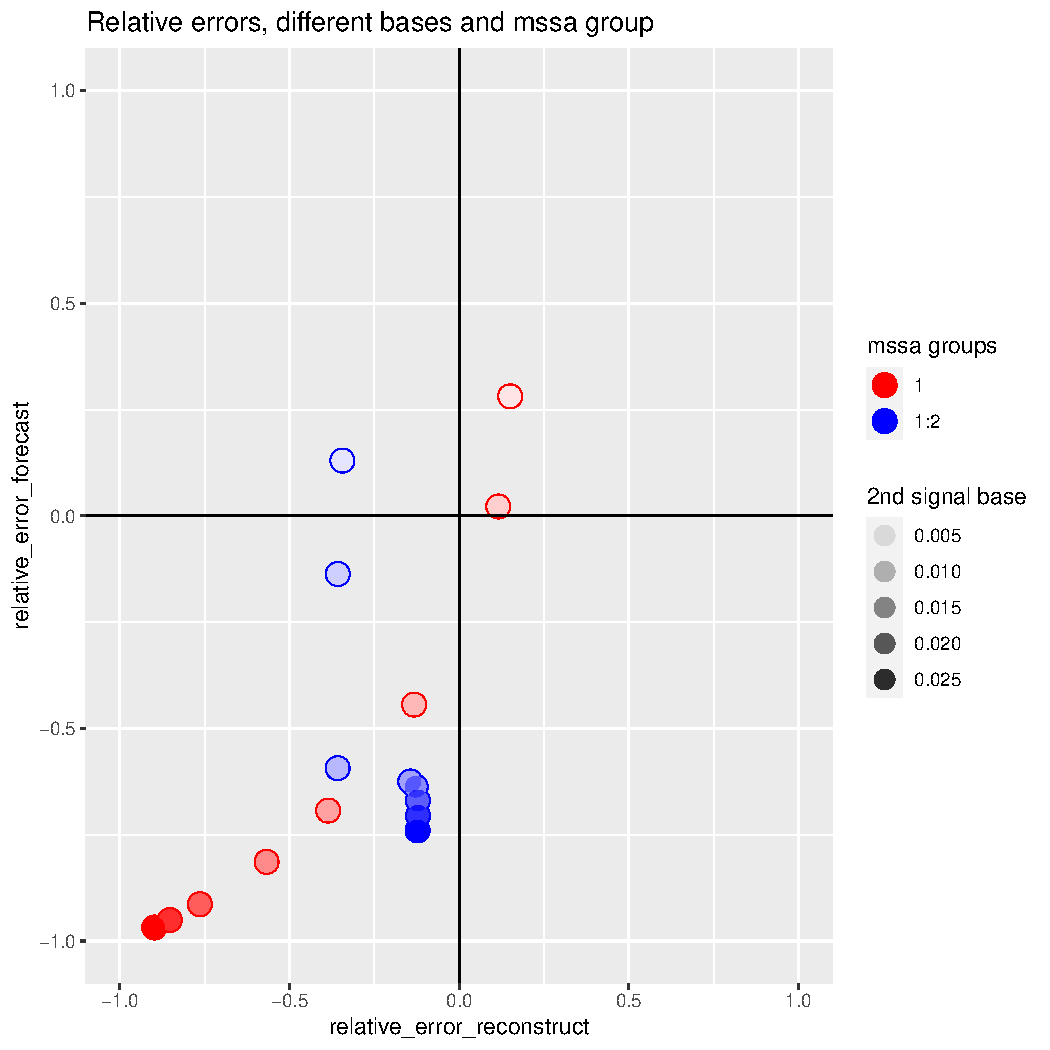
\includegraphics[width=\textwidth]{experiment_1_exp.pdf}
            \caption{Зависимость относительных ошибок от разницы сигналов и выбора ранга для $\MSSA$.}
            \label{fig:exp1_exp}
        \end{figure}

        На рис. \ref{fig:exp1_exp} снова видим подтверждение гипотезы для показательных функций: с увеличением разницы рядов использование двух компонент становится лучше.

    \subsection{Сигнал косинус с показательной модуляцией (общий период, меняющаяся модуляция)}
        Функция для сигналов --- $s^{(i)}_j = A \exp(j\lambda_i) \cos(\frac{2\pi j}{8})$.
        Сигнал $\sfS^{(1)}$ --- функция c $\lambda_1 = 0.005$.
        Сигналы $\sfS^{(2)}$ --- функция c $\lambda_2 \in \{0.005$, $0.0075$, $0.01$, $0.0125$, $0.015$, $0.02$, $0.025$, $0.03\}$.

        Ранг косинуса с модуляцией равен 2, поэтому для $\MSSA$ используются первые 2 или первые 4 компоненты разложения, а для $\SSA$ только 2.

        \begin{figure}[h]
            \centering
            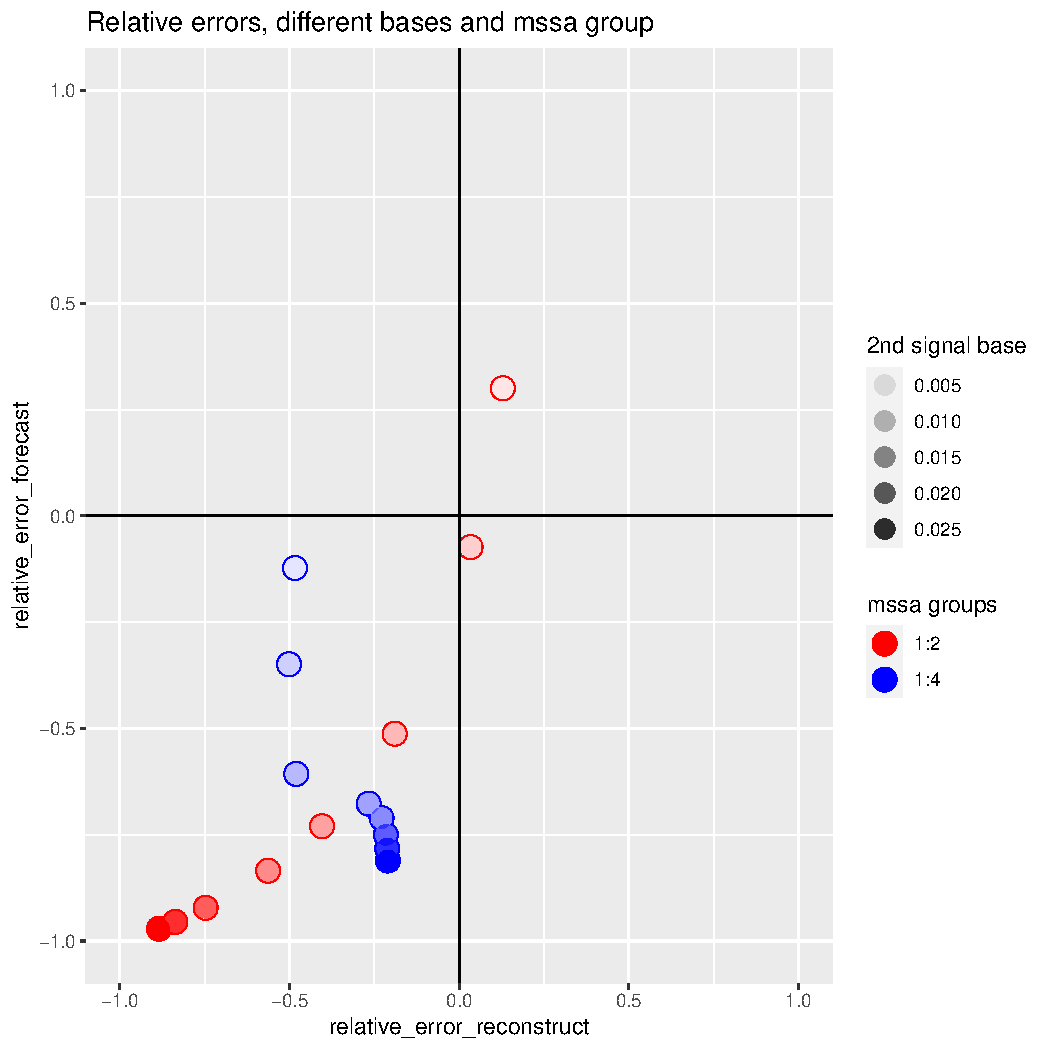
\includegraphics[width=\textwidth]{experiment_1_expcos1.pdf}
            \caption{Зависимость относительных ошибок от разницы сигналов и выбора ранга для $\MSSA$.}
            \label{fig:exp1_expcos1}
        \end{figure}

        На рис. \ref{fig:exp1_expcos1} видим подтверждение гипотезы для косинусов с меняющейся модуляцией.

    \subsection{Сигнал косинус с показательной модуляцией (меняющийся период, общая модуляция)}
        Функция для сигналов --- $s^{(i)}_j = A \exp(0.02j) \cos(\frac{2\pi j}{T_i})$.
        Сигнал $\sfS^{(1)}$ --- функция c $T_1 = 8$.
        Сигналы $\sfS^{(2)}$ --- функция c $T_2 \in \{8$, $8.02$, $8.04$, $8.06$, $8.08$, $8.1$, $8.15\}$.

        Ранг косинуса с модуляцией равен 2, поэтому для $\MSSA$ используются первые 2 или первые 4 компоненты разложения, а для $\SSA$ только 2.

        \begin{figure}[h]
            \centering
            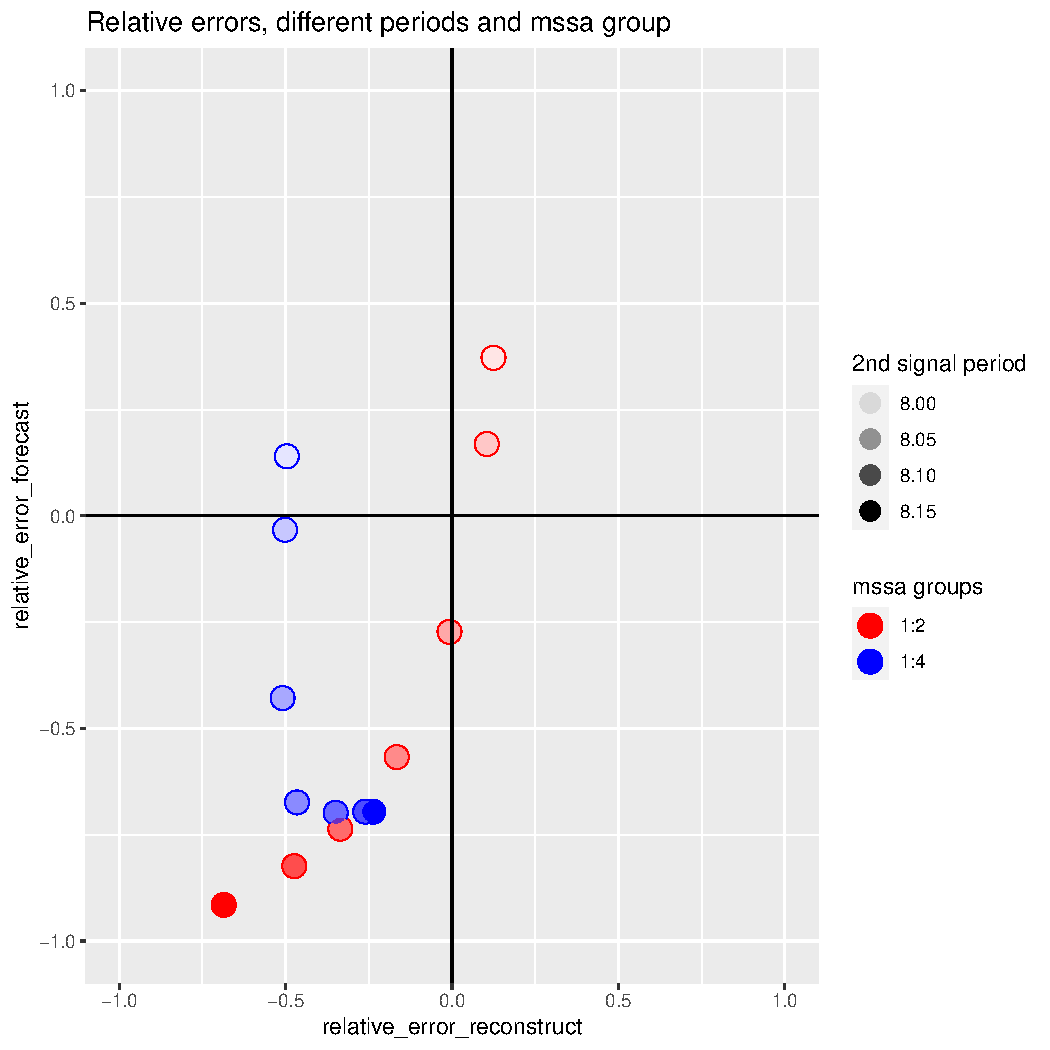
\includegraphics[width=\textwidth]{experiment_1_expcos2.pdf}
            \caption{Зависимость относительных ошибок от разницы сигналов и выбора ранга для $\MSSA$.}
            \label{fig:exp1_expcos2}
        \end{figure}

        На рис. \ref{fig:exp1_expcos2} видим подтверждение гипотезы для модулируемых косинусов с меняющимся периодом.

    \subsection{Результат первого эксперимента}

        Для всех видов сигналов при отклонении второго сигнала от первого всегда наступал момент, когда использование удвоенного ранга дает меньшии ошибки прогноза и восстановления.

        % Так как большая часть наблюдений оказалась в нижней левой четверти графика относительных ошибок, это значит что во всех случаях, кроме $\MSSA$ с маленькой разницей сигналов и рангом равным рангу сигнала, использование $\SSA$ дает лучший результат.

    \section{Второй эксперимент: сравнение ошибки прогноза методами SSA и MSSA при разных величинах шума первого ряда и отклонениях второго ряда}
        Никита Федоров в свей выпускной квалификационной работе изучал влияние величины второго шума на результаты работы $\SSA, \MSSA, \ProjSSA$. Рассмотрим влияние величины первого шума на прогноз $\SSA$ и $\MSSA$, с не зашумленным вторым рядом.

        Гипотеза: при увеличении шума первого ряда, $\MSSA$ станет лучше для любого отклонения второго ряда. Если это так, то можно найти зависимость граничного значения $\sigma_1$ (при котором $\SSA$ становится хуже $\MSSA$) от изменения параметра второго сигнала.

        Как и в первом эксперименте, выберем в качестве первого ряда простой сигнал, зависящий от параметра с аддитивным гауссовым шумом с несколькими значениями дисперсией $\sigma_1^2$.
        Второй ряд будет простым сигналом того же вида, с несколько отличающимся параметром и без шума.
        Спрогнозируем первый ряд с помощью $\SSA$ и $\MSSA$ используя в алгоритме ранг равный рангу сигнала.
        Для устойчивости результатов, повторим это 50 раз и найдем средние ошибки.
        Если графики ошибок прогноза $\SSA$ и $\MSSA$ будут пересекаться, то найдем значения $\sigma_1$ при которых это происходит, это и будут граничные значения $\sigma_1$.

    \subsection{Сигнал косинус}
        Модель сигнала --- $s_j^{(i)} = A \cos(\frac{2\pi j}{T_i})$. Параметры для сигналов: $T_1 = 8$, $T_2 \in \{8$, $8.02$, $8.04$, $8.06$, $8.08$, $8.1$, $8.15\}$, $\sigma_1 \in \{0, 0.1, 0.2, 0.3, 0.4, 0.5, 0.6, 0.7, 0.8, 1\}$, ранг косинуса равен 2.


        \begin{figure}[h]
            \centering
            \begin{minipage}{.5\textwidth}
                \centering
                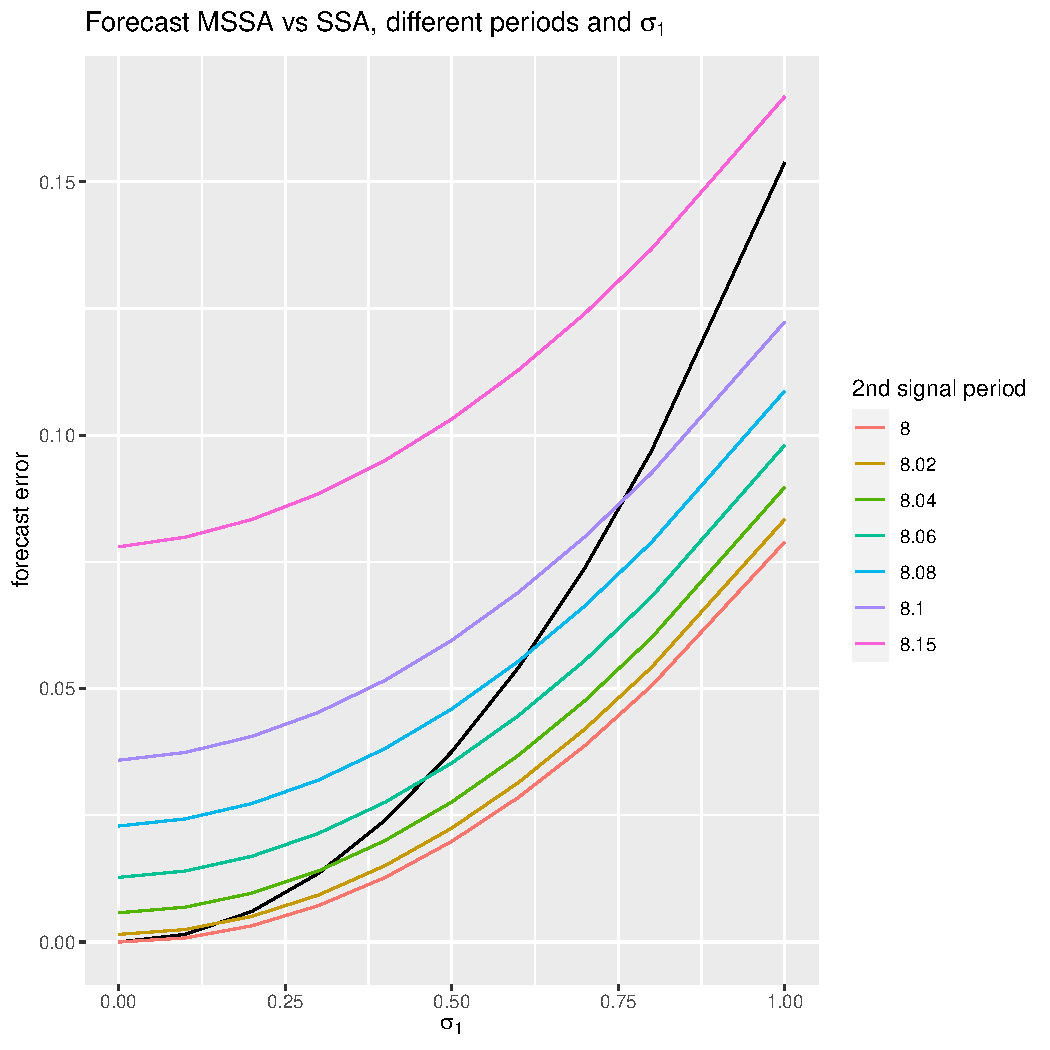
\includegraphics[width=0.9\textwidth]{experiment_2_cos1.pdf}
                \caption{Ошибка прогноза для $\SSA$ и $\MSSA$.}
                \label{fig:exp2_cos1}
            \end{minipage}%
            \begin{minipage}{.5\textwidth}
                \centering
            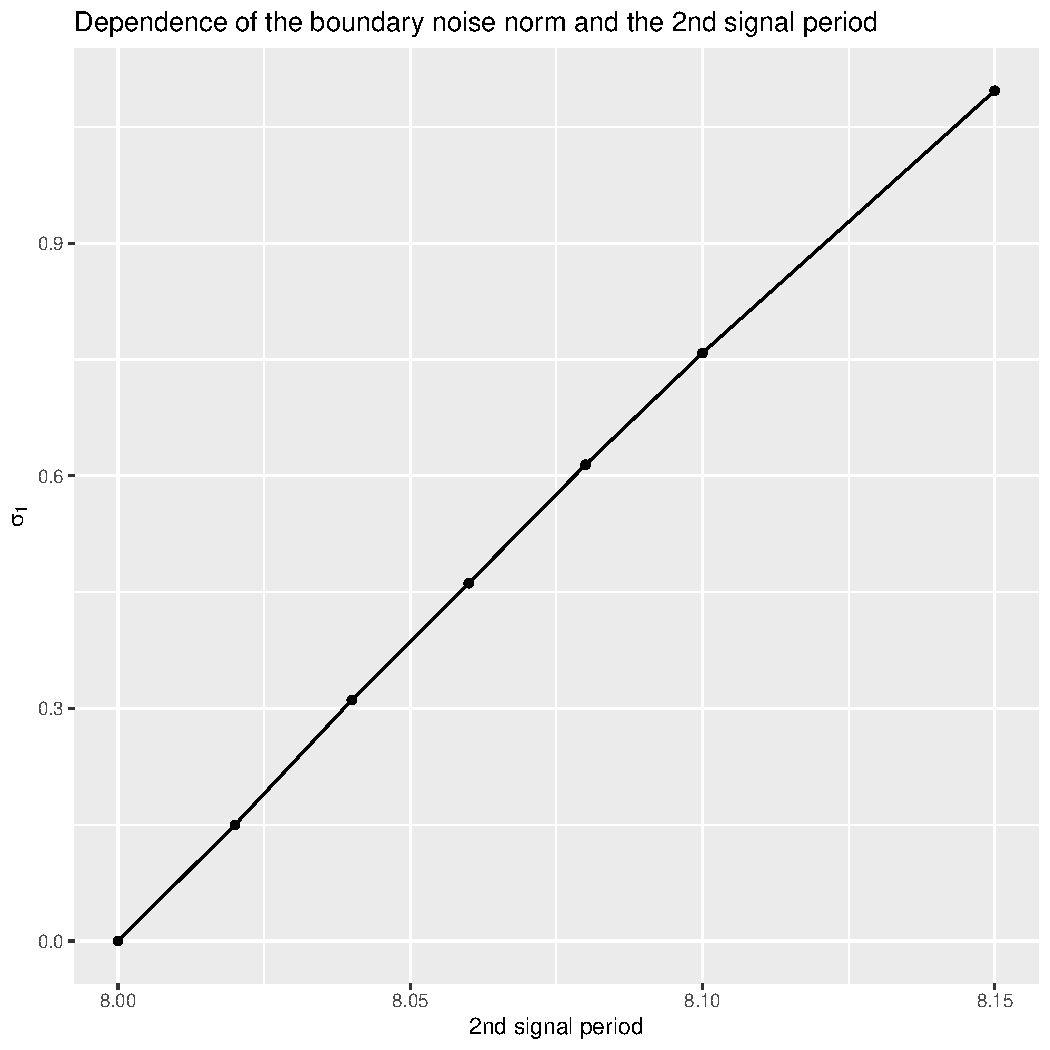
\includegraphics[width=0.9\textwidth]{experiment_2_cos2.pdf}
            \caption{Зависимость граничного значения $\sigma_1$ от второго сигнала}
            \label{fig:exp2_cos2}
            \end{minipage}
        \end{figure}

        На рис. \ref{fig:exp2_cos1} видим, что график ошибки прогноза $\SSA$ (черная линия) пересекает все графики ошибок прогноза $\MSSA$ кроме одного, но они очевидно пересекутся при большем $\sigma_1$. Пересечения графиков будем искать с помощью интерполяции, а для случаев, когда пересечения не было --- с помощью экстраполяции. 

        На рис. \ref{fig:exp2_cos2} изображены полученные граничные значения $\sigma_1$ для каждого второго сигнала. Видна линейная зависимость.

    \subsection{Сигнал экспонента (показательная функция)}
        Модель сигнала --- $s^{(i)}_j = A \exp(j\lambda_i)$. Параметры для сигналов: $\lambda_1 = 0.005$, $\lambda_2 \in \{0.005$, $0.01$, $0.012$, $0.013$, $0.015$, $0.0175$, $0.02\}$, $\sigma_1 \in \{0, 0.3, 0.6, 1, 1.5, 2\}$, ранг косинуса равен 2.


        \begin{figure}[h]
            \centering
            \begin{minipage}{.5\textwidth}
                \centering
                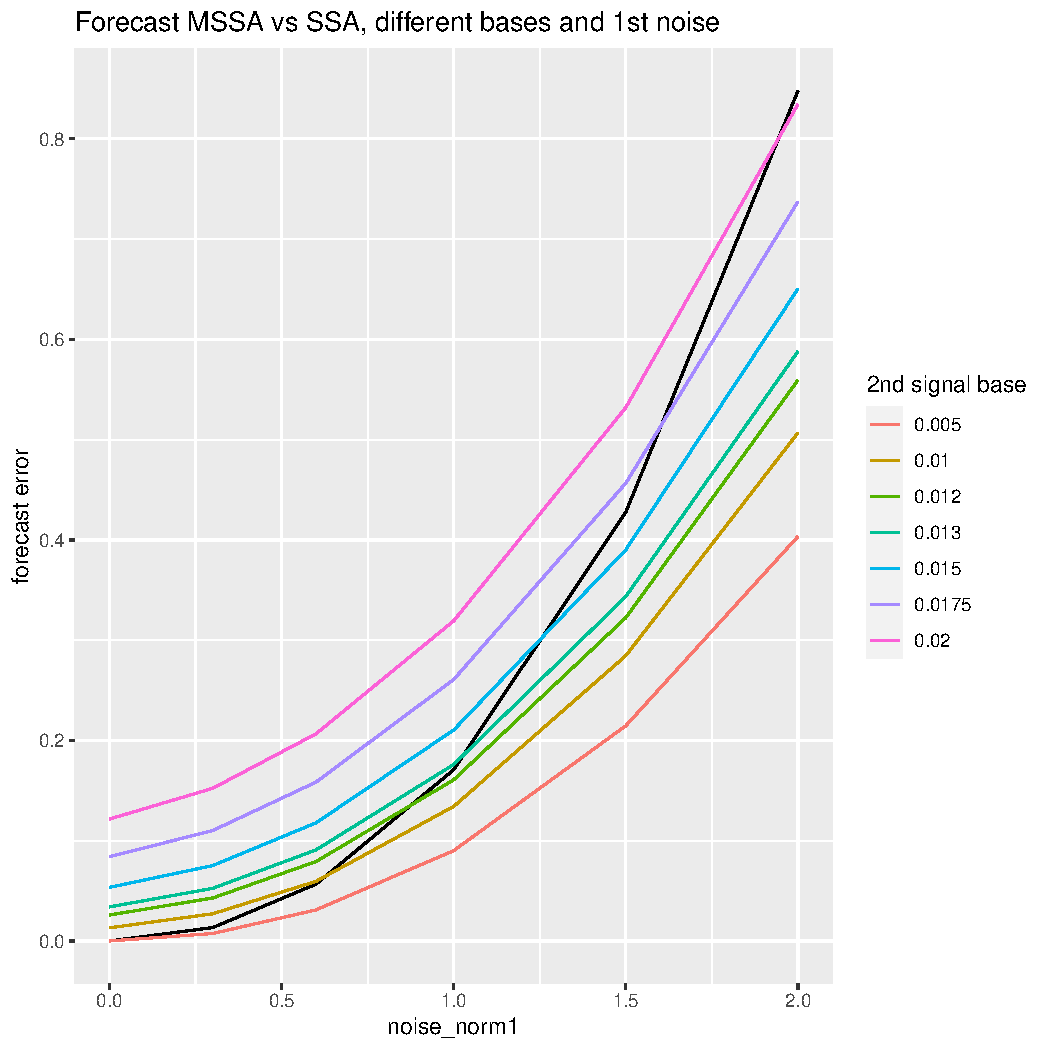
\includegraphics[width=0.9\textwidth]{experiment_2_exp1.pdf}
                \caption{Ошибка прогноза для $\SSA$ и $\MSSA$.}
                \label{fig:exp2_exp1}
            \end{minipage}%
            \begin{minipage}{.5\textwidth}
                \centering
            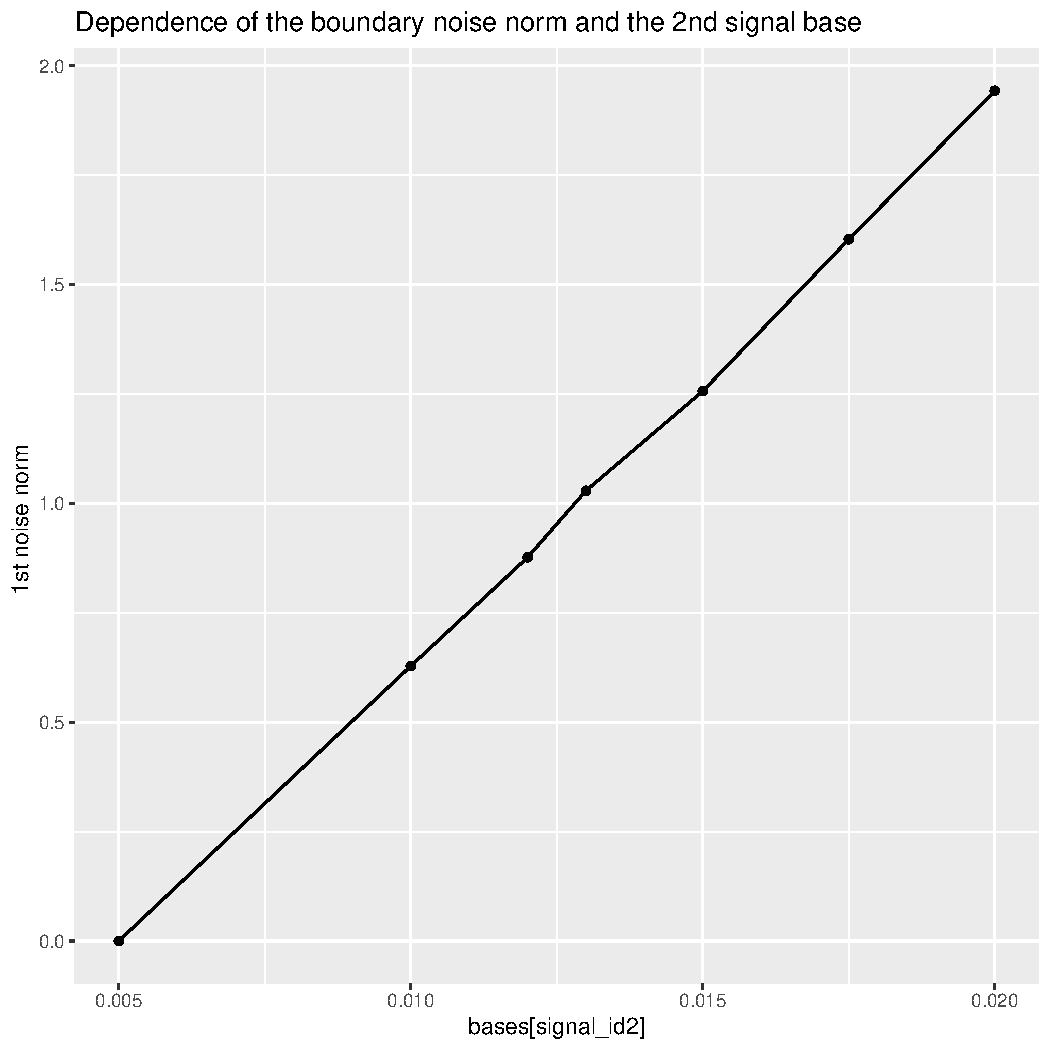
\includegraphics[width=0.9\textwidth]{experiment_2_exp2.pdf}
            \caption{Зависимость граничного значения $\sigma_1$ от второго сигнала}
            \label{fig:exp2_exp2}
            \end{minipage}
        \end{figure}

        На рис. \ref{fig:exp2_exp1} видим, что график ошибки прогноза $\SSA$ (черная линия) пересекает все графики ошибок прогноза $\MSSA$. 

        На рис. \ref{fig:exp2_exp2} видна линейная зависимость, как с косинусом.
    
    \subsection{Результат второго эксперимента}
        Гипотеза подтверждена, зависимость граничных значений $\sigma_1$ от отклонения второго сигнала линейная или очень близка к линейной.

    \section{Третий эксперимент: линейные сигналы}

        \begin{figure}[h]
            \centering
            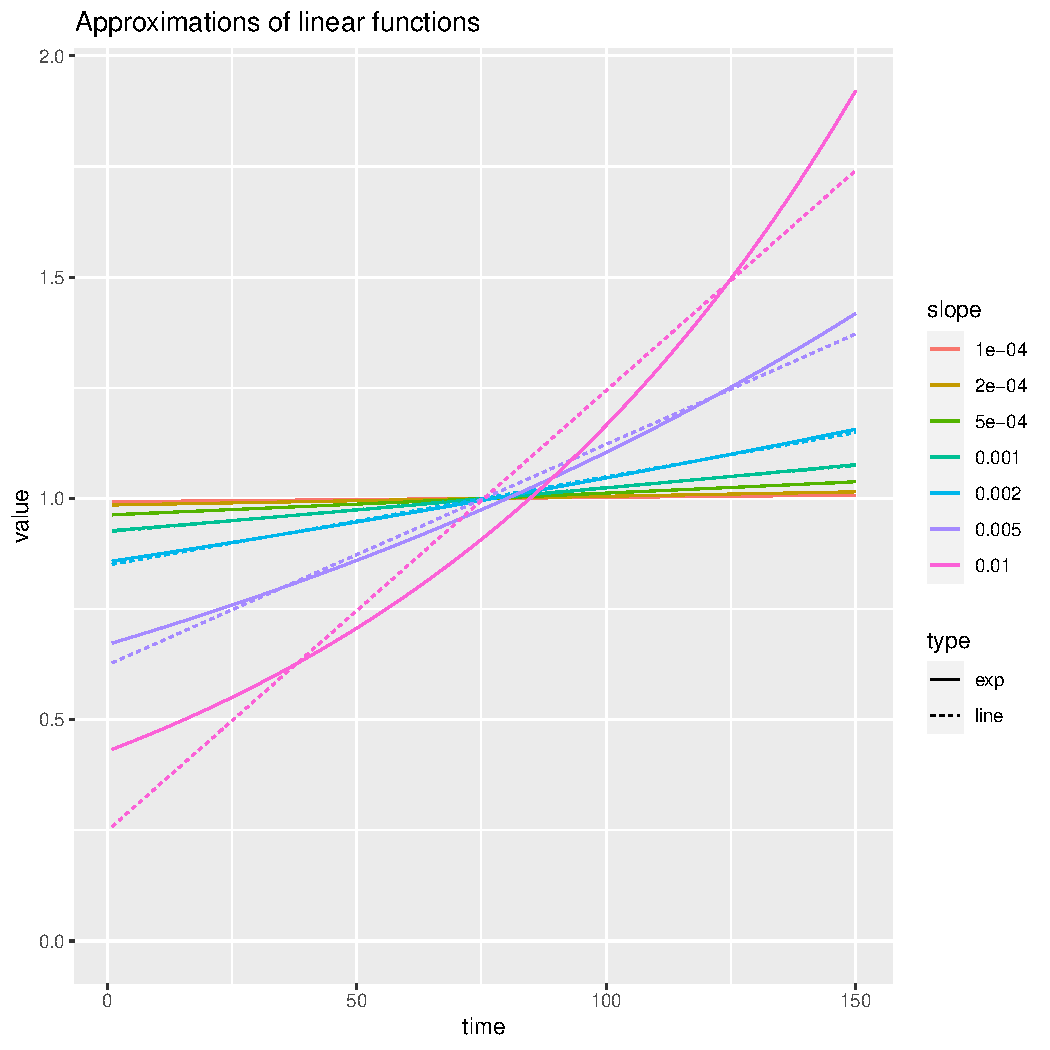
\includegraphics[width=0.8\textwidth]{experiment_3_expline.pdf}
            \caption{Пример аппроксимации линейных функций показательными.}
            \label{fig:exp3_expline}
        \end{figure}

        Как видно на рис. \ref{fig:exp3_expline} иногда линейный сигнал можно хорошо аппроксимировать показательной функцией. Причем, качество приближения зависит от угла наклона. Из-за того, что ранг линейного сигнала равен 2, а показательного --- 1, становится интересно, можно ли использовать экспоненциальный сигнал как поддерживающий для линейного?

    \subsection{Является ли первая компонента разложения линейного ряда показательной функцией?}
        Для того чтобы понять можно ли использовать экспоненциальный сигнал как поддерживающий для линейного, нужно узнать, на сколько их структура похожа. Например, сравнить аппроксимацию линейного сигнала рядом ранга 1 (восстановить первую компоненту алгоритмом $\SSA$) и аппроксимацию этого же сигнала экспоненциальной функцией.

        \begin{figure}[h]
            \centering
            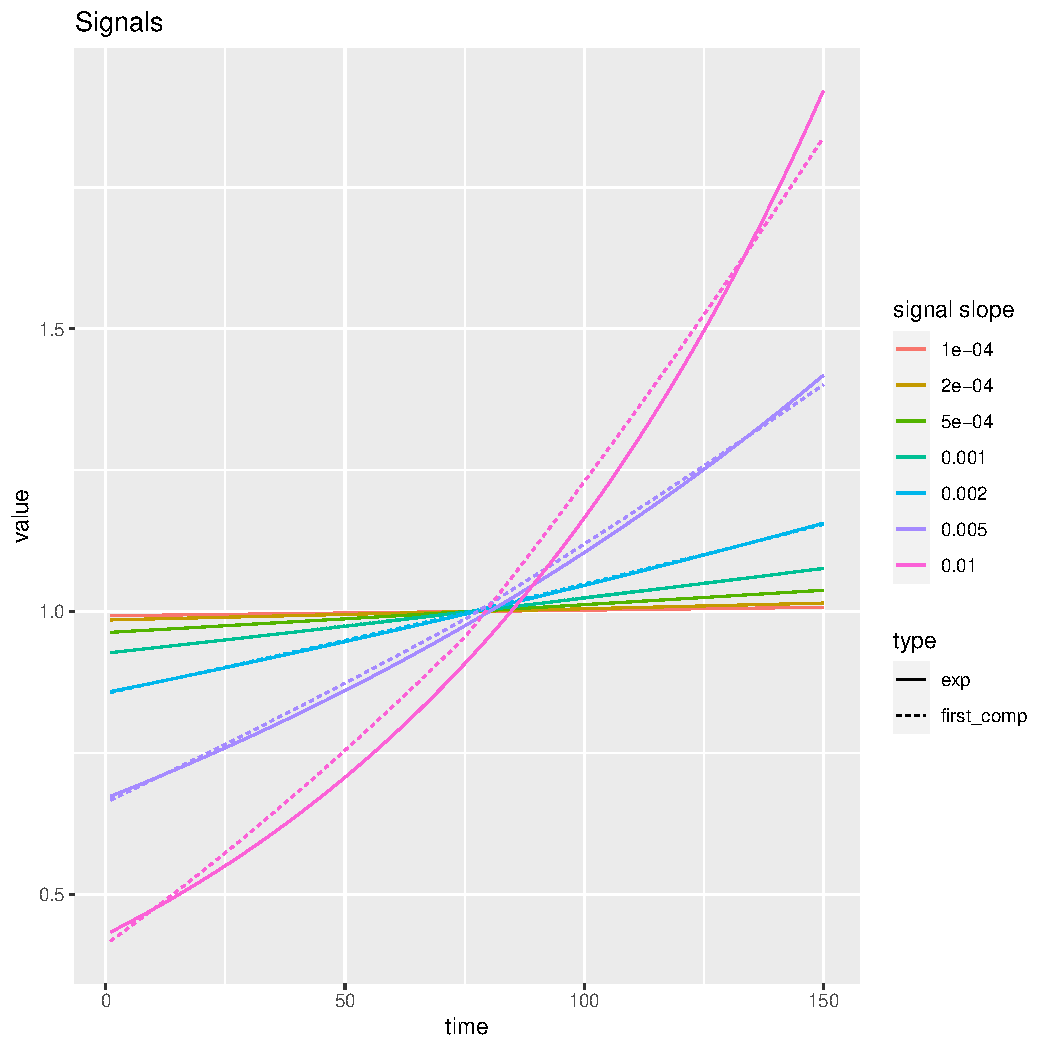
\includegraphics[width=0.8\textwidth]{experiment_3_linefirstcomp.pdf}
            \caption{Сравнение первых компонент сигнала и аппроксимирующих экспонент.}
            \label{fig:exp3_linefirstcomp}
        \end{figure}

        Из рис. \ref{fig:exp3_linefirstcomp} видно что первая компонента разложения линейного ряда не является показательной функцией, так как показательные функции не могут дважды пересекаться.

    \subsection{Зависимость доли второй компоненты от угла наклона}

        Как уже было замечено, при меньших углах наклона, аппроксимация получается лучше. Есть ли зависимость доли второй компоненты в линейном сигнале от угла наклона?

        
        \begin{figure}[h]
            \centering
            \begin{minipage}{.5\textwidth}
                \centering
                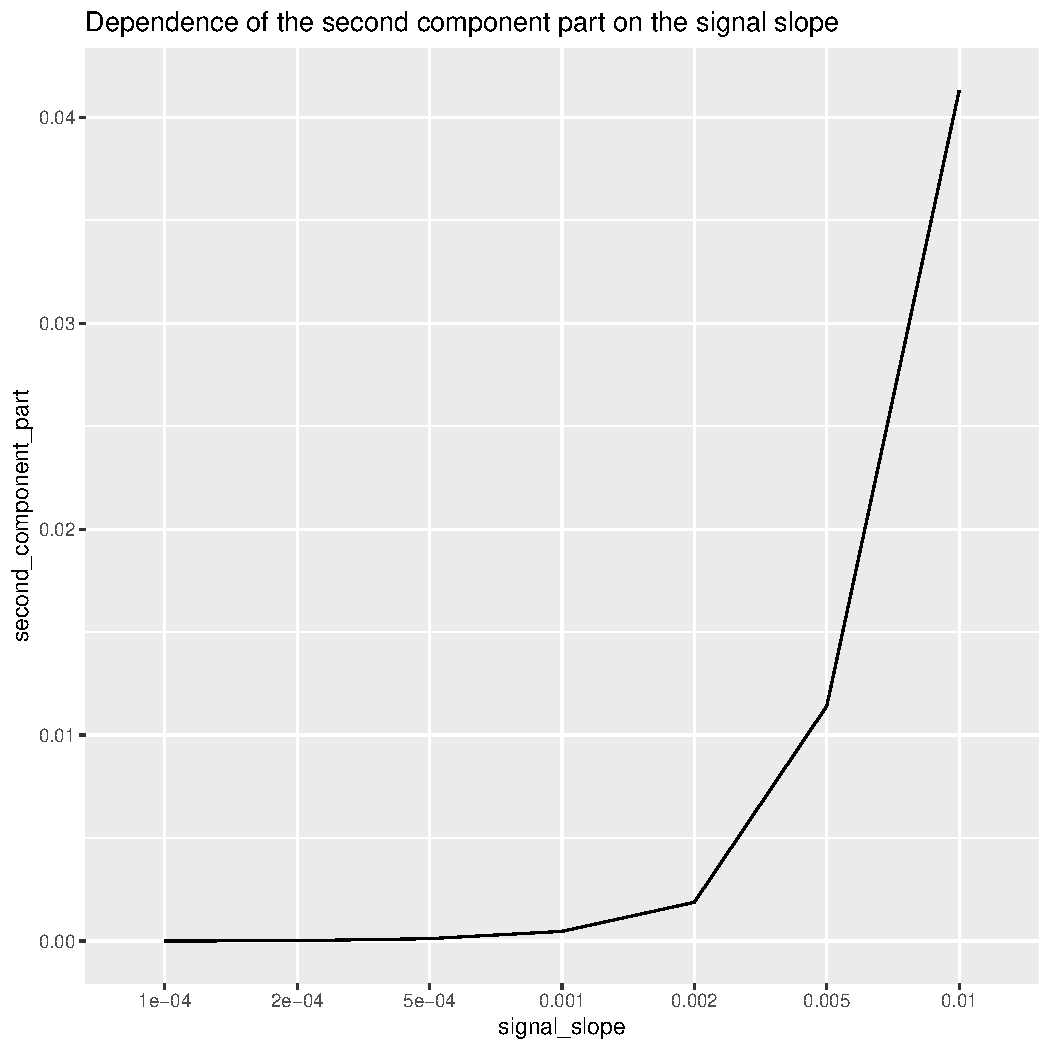
\includegraphics[width=0.9\textwidth]{experiment_3_secondpart1.pdf}
                \caption{Зависимость доли второй компоненты от угла наклона линейного сигнала.}
                \label{fig:exp3_secondpart1}
            \end{minipage}%
            \begin{minipage}{.5\textwidth}
                \centering
            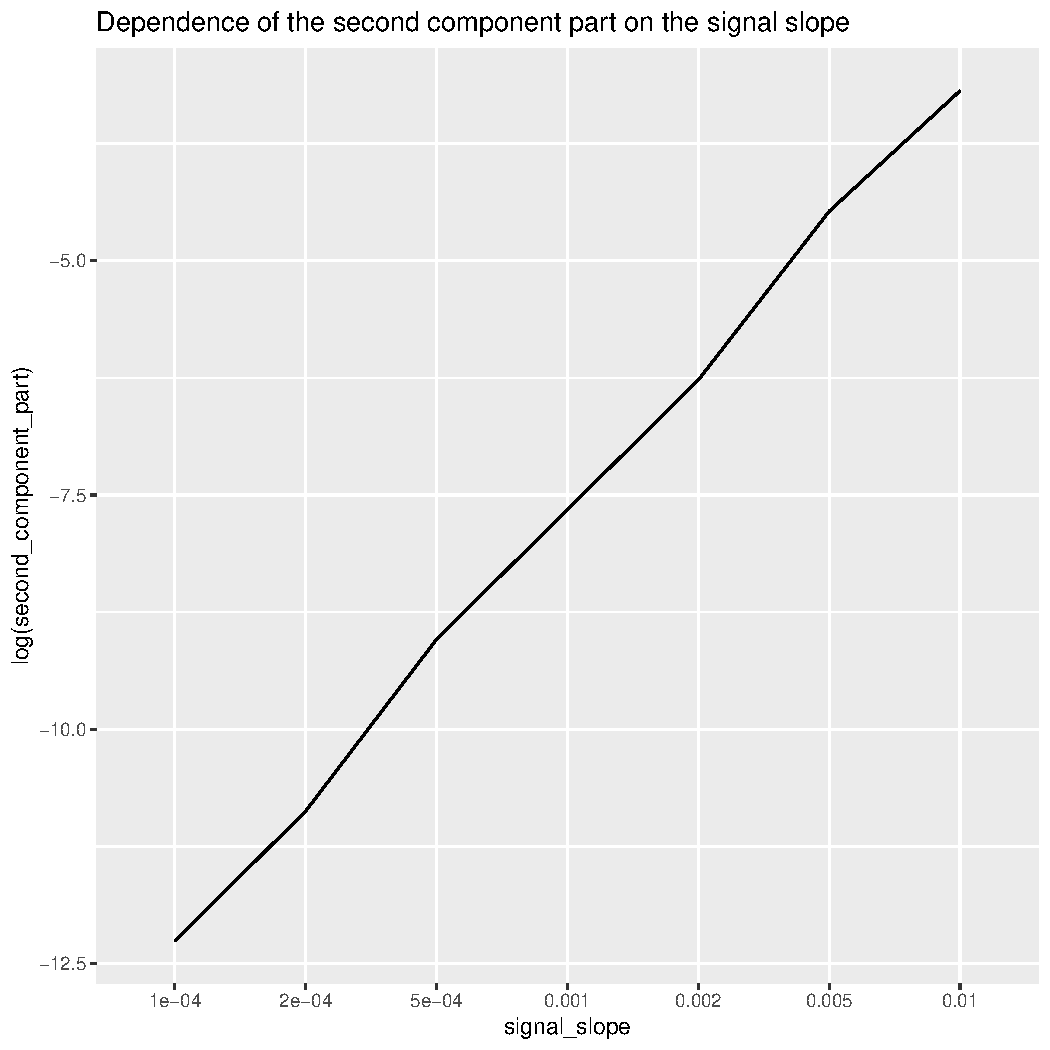
\includegraphics[width=0.9\textwidth]{experiment_3_secondpart2.pdf}
            \caption{Зависимость логарифма доли второй компоненты от угла наклона линейного сигнала.}
            \label{fig:exp3_secondpart2}
            \end{minipage}
        \end{figure}


        % \begin{figure}[h]
        %     \centering
        %     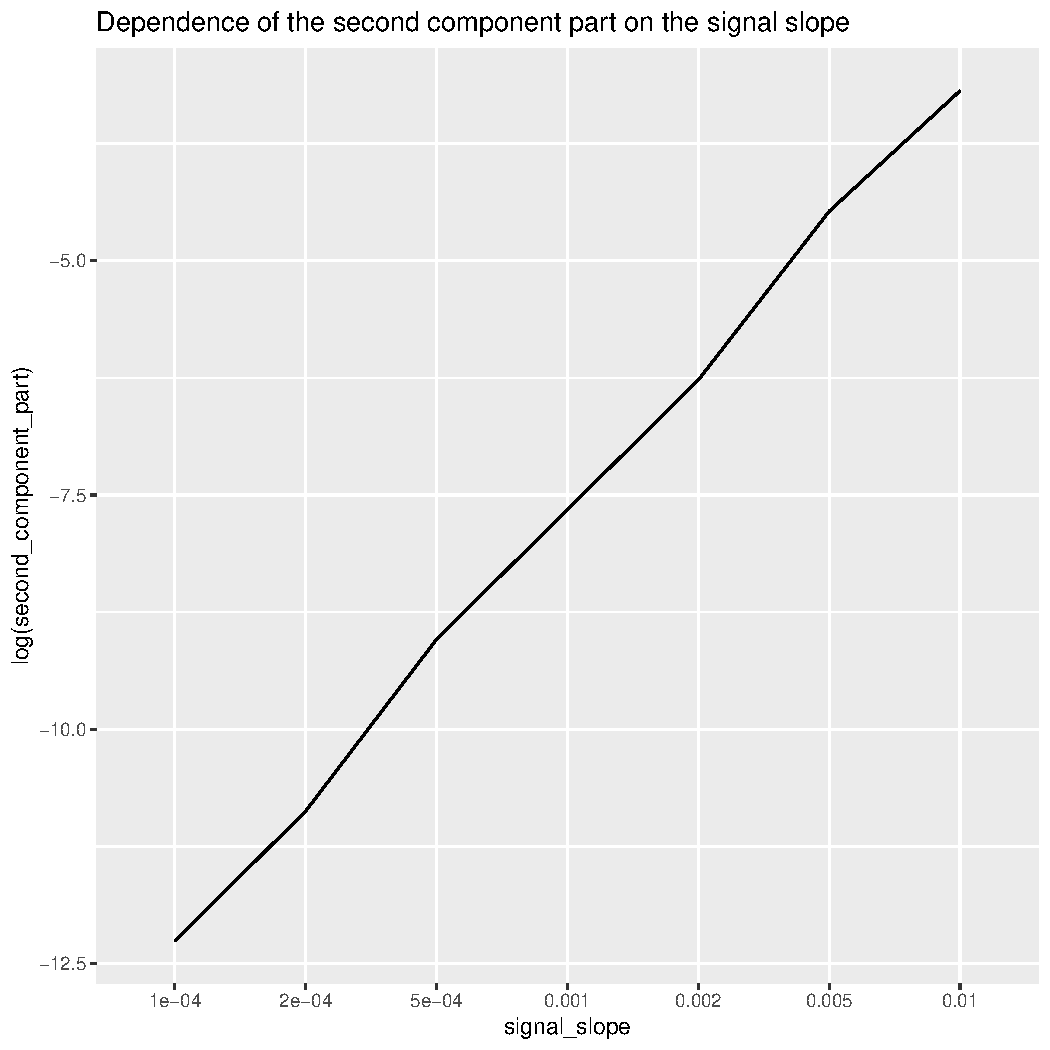
\includegraphics[width=0.8\textwidth]{experiment_3_secondpart.pdf}
        %     \caption{Зависимость доли второй компоненты от угла наклона линейного сигнала.}
        %     \label{fig:exp3_secondpart}
        % \end{figure}

        На рис. \ref{fig:exp3_secondpart1} зависимость похожа на экспоненциальную, прологарифмируем и проверим это.
        На рис. \ref{fig:exp3_secondpart2} видна линейная зависимость логарифма доли второй компоненты и угла наклона сигнала, поэтому доля второй компоненты действительно зависит экспоненциально от угла наклона.

    \subsection{При каком шуме вторая компонента теряется}
        На рис. \ref{fig:exp3_secondpart1} можно заметить, что доля второй компоненты мала, а значит в алгоритме $\SSA$ она может оказаться не второй и быть потеряна при достаточно большом шуме.

        Как понять, что вторая компонента потерялась не изучая разложение в ручную?
        
        Будем восстанавливать одну или две компоненты алгоритмом $\SSA$ из линейных сигналов с разными углами наклона и считать ошибку восстановления. Когда вторая компонента теряется, ошибка двух компонент становится больше ошибки одной компоненты, потому что вместо нужной второй компоненты ряда берется часть шума.
        
        \begin{figure}[h]
            \centering
            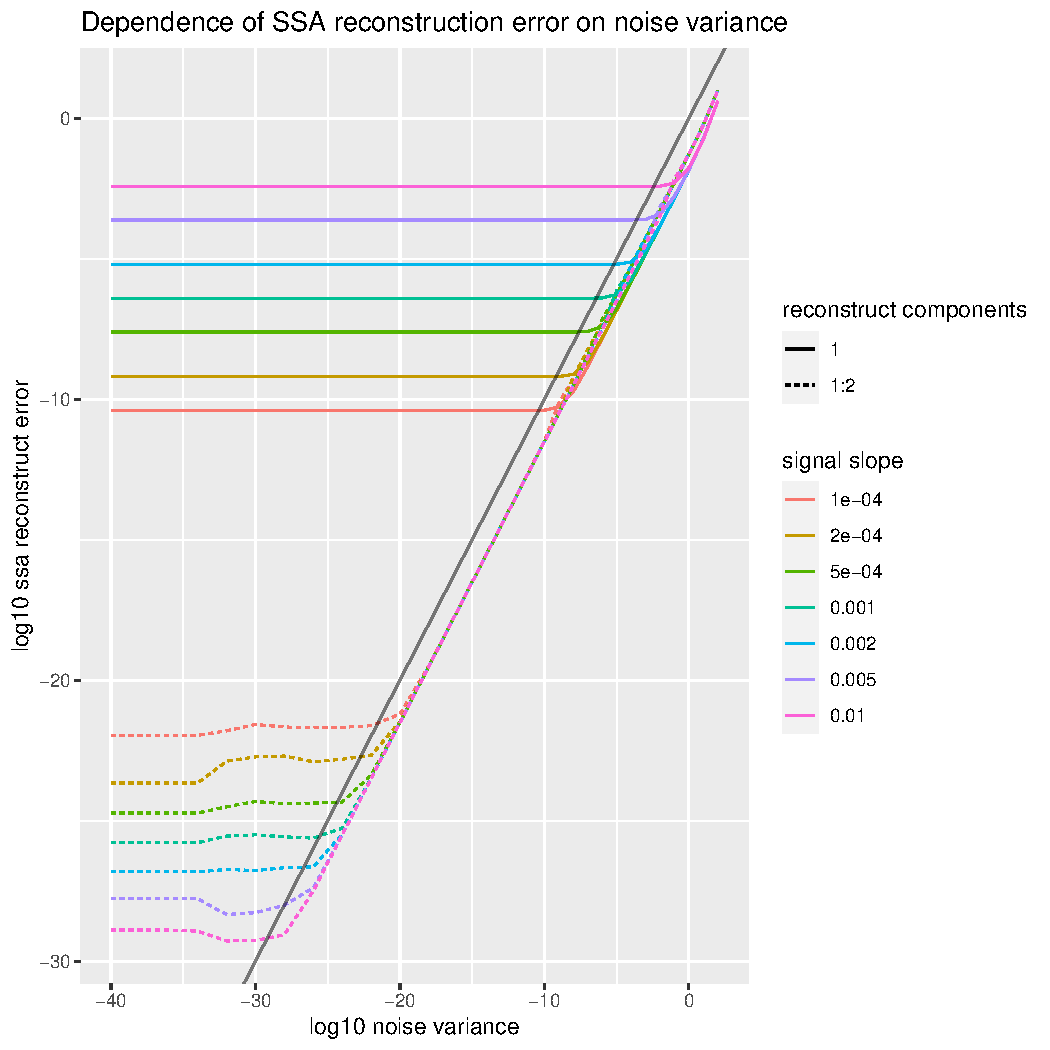
\includegraphics[width=0.8\textwidth]{experiment_3_lost1.pdf}
            \caption{Зависимость ошибки восстановления от $\sigma^2$.}
            \label{fig:exp3_lost1}
        \end{figure}

        \begin{figure}[h]
            \centering
            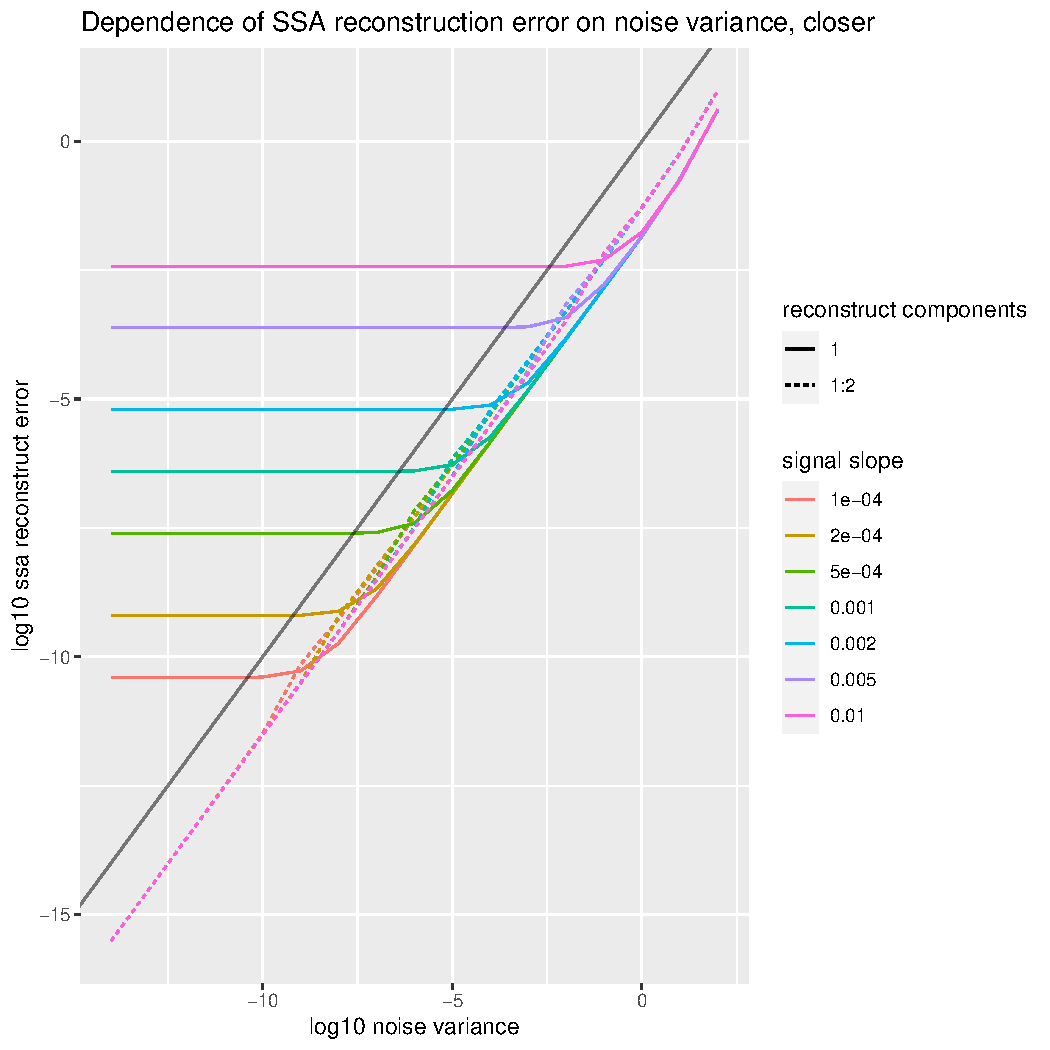
\includegraphics[width=0.8\textwidth]{experiment_3_lost2.pdf}
            \caption{Зависимость ошибки восстановления от $\sigma^2$, крупнее.}
            \label{fig:exp3_lost2}
        \end{figure}

        На рис. \ref{fig:exp3_lost1} и \ref{fig:exp3_lost2} черная линия показывает прямую $x = y$, цветные линии --- графики ошибок восстановления, пунктирные --- двумя компонентами, сплошные --- одной. Чтобы ответить на поставленный вопрос, найдем точки пересечения графиков с помощью интерполяции и построим график.

        \begin{figure}[h]
            \centering
            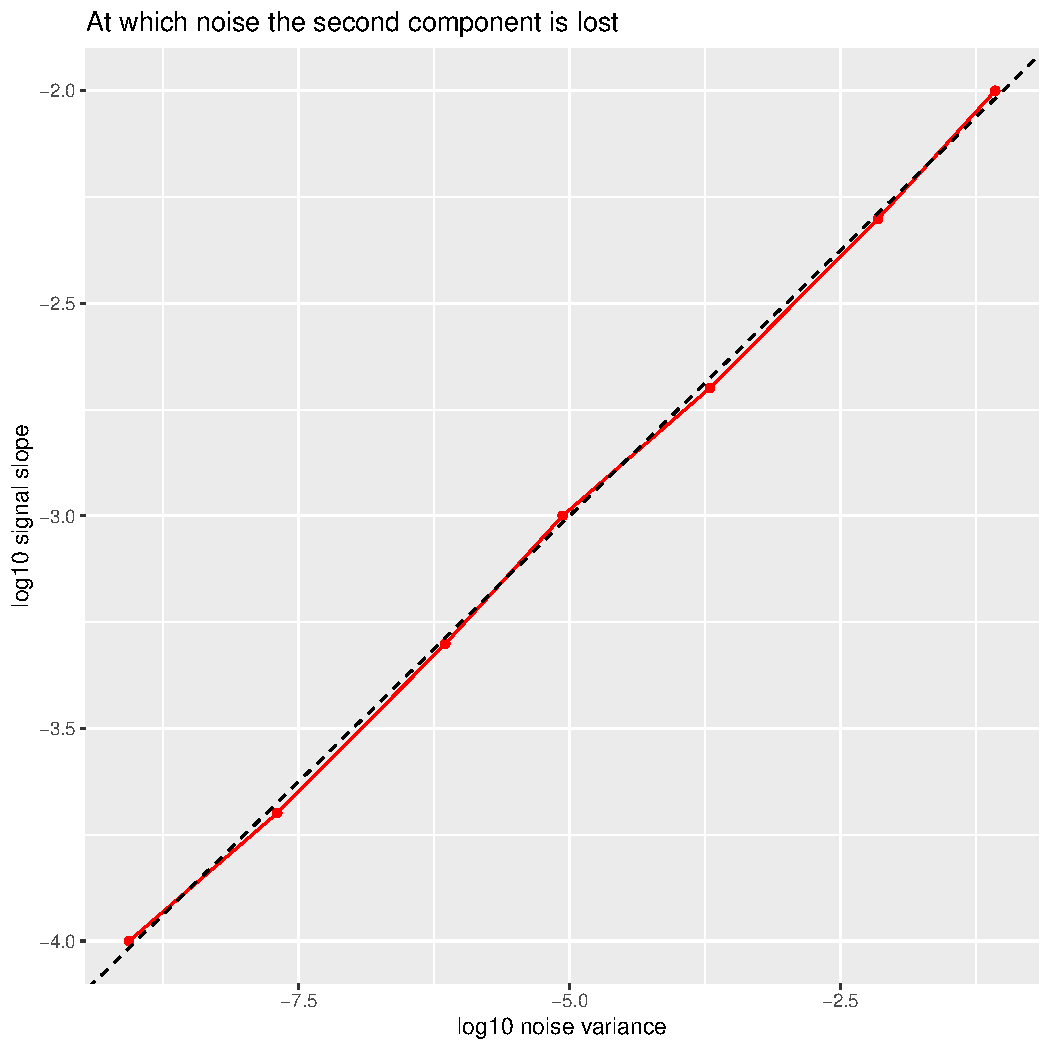
\includegraphics[width=0.8\textwidth]{experiment_3_lost3.pdf}
            \caption{Зависимость ошибки восстановления от $\sigma^2$}
            \label{fig:exp3_lost3}
        \end{figure}

        На рис. \ref{fig:exp3_lost3} черным пунктиром обозначена прямая $4y = x - 7$. Зависимость логарифмов угла наклона и дисперсии шума близка к уравнению $4\log_{10}(slope) = \log_{10}(\sigma^2) - 7$, поэтому сама зависимость выражается уравнением $slope^4 = 10^{-7}\sigma^2$.

        % \subsection{Результат третьего эксперимента}



        % линейный сигнал раскладывается на 2 компоненты, доля второй маленькая, и может потеряться в шуме...
        

        % теперь узнать при каком шуме вторая компонента потеряется
        % красивый график + ответ на вопрос
        



    % \section{старое}
    %     Выдвинута гипотеза, что ряд $\F^{(2)}$ поддерживающий для ряда $\F^{(1)}$, если их сигналы $\sfS^{(1)}$, $\sfS^{(2)}$ согласованны и шум $\sfR^{(2)}$ небольшой.

    %     Так как на практике могут встречаться отклонения от полностью согласованных сигналов, хочется узнать, на сколько можно исказить сигнал второго ряда, прежде чем он перестанет быть поддерживающим?

    %     Для подтверждения гипотезы и ответа на вопрос была проведена серия описанных ниже экспериментов.

    %     Временные ряды строились как сумма сигнала и шума.
    %     В качестве моделей сигнала использовались функции из списка:
    %         \begin{enumerate}
    %             \item $s^{(i)}_j = \exp(j\lambda_i);$
    %             \item $s^{(i)}_j = \cos(\frac{2\pi j}{12})\exp(j\lambda_i);$
    %             \item $s^{(i)}_j = \cos(\frac{2\pi j}{T_i});$
    %             \item $s^{(i)}_j = \cos(\frac{2\pi j}{12}) + \exp(j\lambda_i).$
    %         \end{enumerate}
    %     Параметр первого сигнала (период косинуса $T_1$ или база показательный функции $\lambda_1$) фиксировался, параметр второго сигнала менялся, начиная с такого же значения как у первого, до момента, когда второй ряд переставал быть поддерживающим.
    %     В качестве шума для обоих рядов использовались независимые белые гауссовские шумы со средними, равными 0, и дисперсиями $\sigma_1^2, \sigma_2^2$, соответственно.



    % \section{старые Результаты}
        
    %     Гипотеза была подтверждена для всех четырех моделей сигнала. Ряд, сигнал которого полностью согласован с сигналом прогнозируемого, перестает быть поддерживающим, если его шум слишком большой.

    %     Показательные функции, умноженные на косинус с общим периодом, оставались поддерживающими дольше, чем показательные функции без косинусов.
    %     Показательные функции, к которым был прибавлен косинус, тоже были поддерживающими дольше, чем показательные функции без косинусов.
        


    \conclusion
        Найдено много интересных зависимостей, характер и причины которых еще предстоит объяснить.

        В дальнейшем планируется изучить использование экспоненциального ряда в качестве поддерживающего для линейного и наоборот.
 

        
        % \begin{itemize}
        %     \item Как по структуре рядов понять согласованность?
        %     \item Что если ранги рядов разные?
        % \end{itemize}

    
    % \section{Литература}
	% \nocite{L1}

	\renewcommand{\refname}{}
	\vspace{-25pt}
	\bibliographystyle{ugost2008}
	\bibliography{references}
\end{document}